\documentclass[11pt]{article}

\usepackage[tmargin=1in,bmargin=1in]{geometry}
\usepackage{amsmath, amssymb, amsthm}
\usepackage{enumitem}
\usepackage{multicol}
\usepackage{graphicx}

\graphicspath{./}

\usepackage{helvet}
\renewcommand{\familydefault}{\sfdefault}

\title{Statistical Analysis of the Virtual Safety Car in Formula One}
\date{}

\begin{document}

\maketitle
\paragraph*{Abstract}
This paper reviews the potential statistical impacts that the Virtual Safety Car has on actual Safety Car Deployments in Formula One.

\pagebreak

\section{Introduction}
In Formula One cars and drivers speed around a racetrack, occasionally creating accidents or situations that require caution. In 2015 Formula One introduced the Virtual Safety Car (VSC). Instead of deploying a physical safety car, a ``virtual'' safety car can be deployed to automatically slow down drivers when necessary. This paper analyzes the impact that the VSC may have had on actual safety car deployments.

\section{Data}
This paper analyzes data provided by Kaggle with supplementary stats compiled manually.
\begin{description}
    \item[Year] Year at which the race took place.
    \item[Race] Name of the race.
    \item[Type] Permanent (racing facility) or Street (street circuit).
    \item[Round] The n-th round of the season (year).
    \item[TotalRounds] Number of races for that season (year).
    \item[TotalLaps] Total number of laps completed for that race.
    \item[Condition] Dry (dry track), Mixed (mixed condition of dry and wet), or Wet (wet track)
    \item[Cause] Cause of deploying the safety car.
    \item[Deployed] The lap at which the safety car was deployed.
    \item[Retreated] The lap at which the safety car returned to the pit lane. If empty, the race had a safety car finish.
    \item[FulllLaps] The number of laps led by the safety car.
\end{description}

\section{Method}
The data was analyzed using the R programming language to generate visual graphs and numerical comparisons. A histogram was generated for Formula One season 2010-2015 and 2015-2019 with a best-fit poisson line overlayed.
Similarly, the interval between safety car deployments was graphed with a best-fit exponential line overlayed.
Lastly, we conducted two-sample t-tests comparing both intervals, one with variance assumed equal and one without.

\pagebreak

\section{Results}

Looking first at the means and standard deviations of the two samples, we see that the mean (\# of safety car deployments) of the 2010-2015 sample is 0.7291667 and the standard deviation is 1.061074.

\begin{figure}[h]
    \centering
    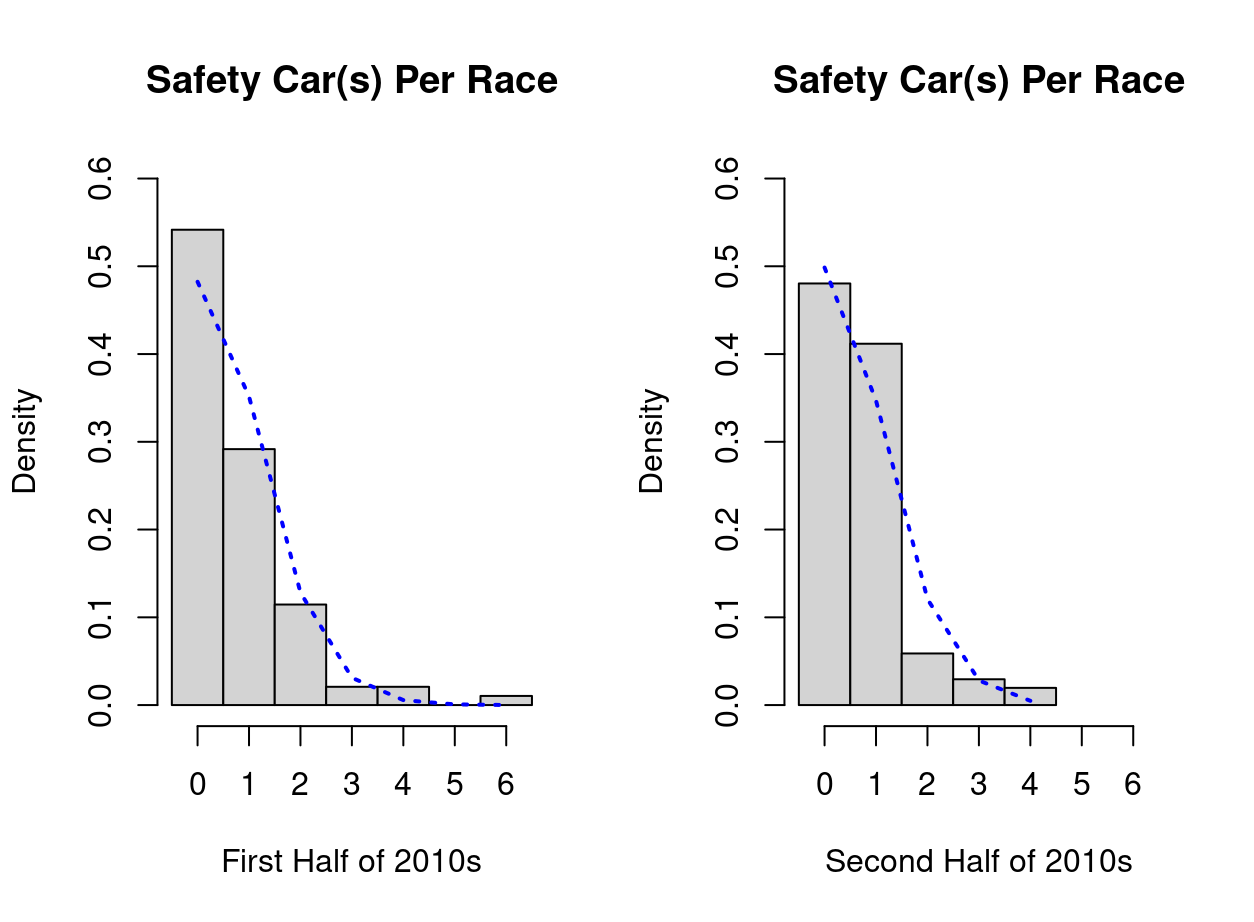
\includegraphics[width=0.5\textwidth]{deployment-histogram.png}
    \caption{Histogram of Safety Car Deployments}
    \label{fig:histogram}
\end{figure}

The mean of the 2015-2019 sample is 0.6960784 and the standard deviation is 0.8650441.
We can see the histogram of deployments in Figure \ref{fig:histogram}.

\begin{figure}[h]
    \centering
    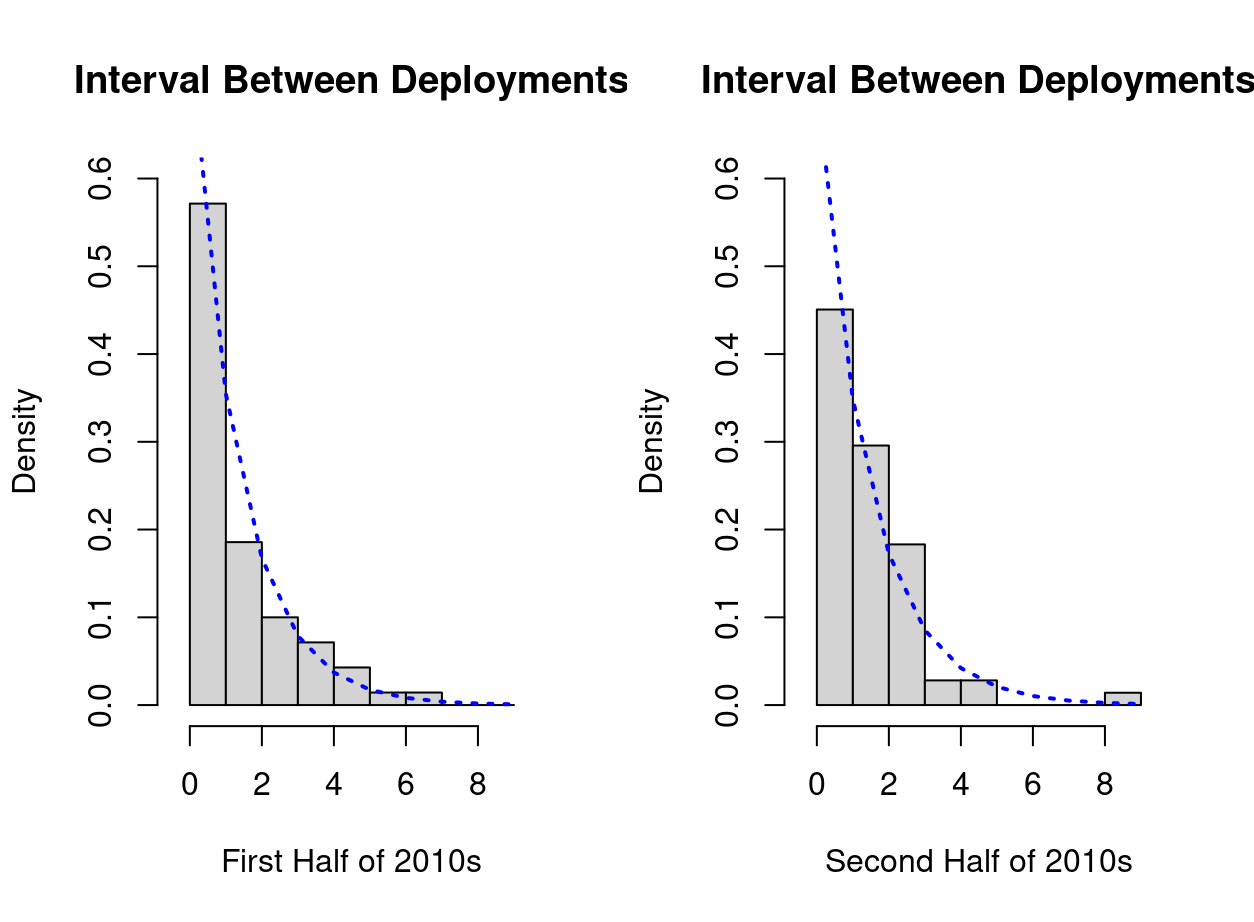
\includegraphics[width=0.5\textwidth]{interval-histogram.png}
    \caption{Histogram of Safety Car Intervals}
    \label{fig:interval}
\end{figure}

Similarly, the mean of the intervals between deployments for 2010-2015 is 1.328827 vs 1.421543 for 2015-2019.
We can see the histogram of intervals in Figure \ref{fig:interval}.

\pagebreak

Finally, we conducted two-sample t-tests comparing both intervals, one with variance assumed equal and one without.

\subsection*{\rightline{Assuming Equal Variance}}
\begin{align*}
    t              & = -0.39129 \\
    df             & = 139      \\
    p\text{-}value & = 0.6962
\end{align*}

Which generated a p-value of 0.6962, indicating that the two samples are not significantly different.
More specifically, the 95\% confidence interval for the difference in means is [-0.5612108, 0.3757772].

\subsection*{\rightline{Not Assuming Equal Variance}}
\begin{align*}
    t              & = -0.39133 \\
    df             & = 139      \\
    p\text{-}value & = 0.6962
\end{align*}

Which generated a p-value of 0.6962, the same as the previous test.
Lastly, the 95\% confidence interval for the difference in means is [-0.5611611, 0.3757275].

\section*{Conclusion}
Going by our t-tests and visually comparing histograms, we can conclude that there is not a significant impact on safety car deployments due to the introduction of the VSC.

\end{document}